\subsection{Bestimmung der Ankerinduktivität}

Um die Ankeridnuktivität zu bestimmen muss der Motor gebremst sein,
damit die induzierte Gegenspannung $U_{ind} = 0$ ist. Dann ergibt sich
folgendes Schaltbild.


\begin{figure}[H]
    \centering
   %  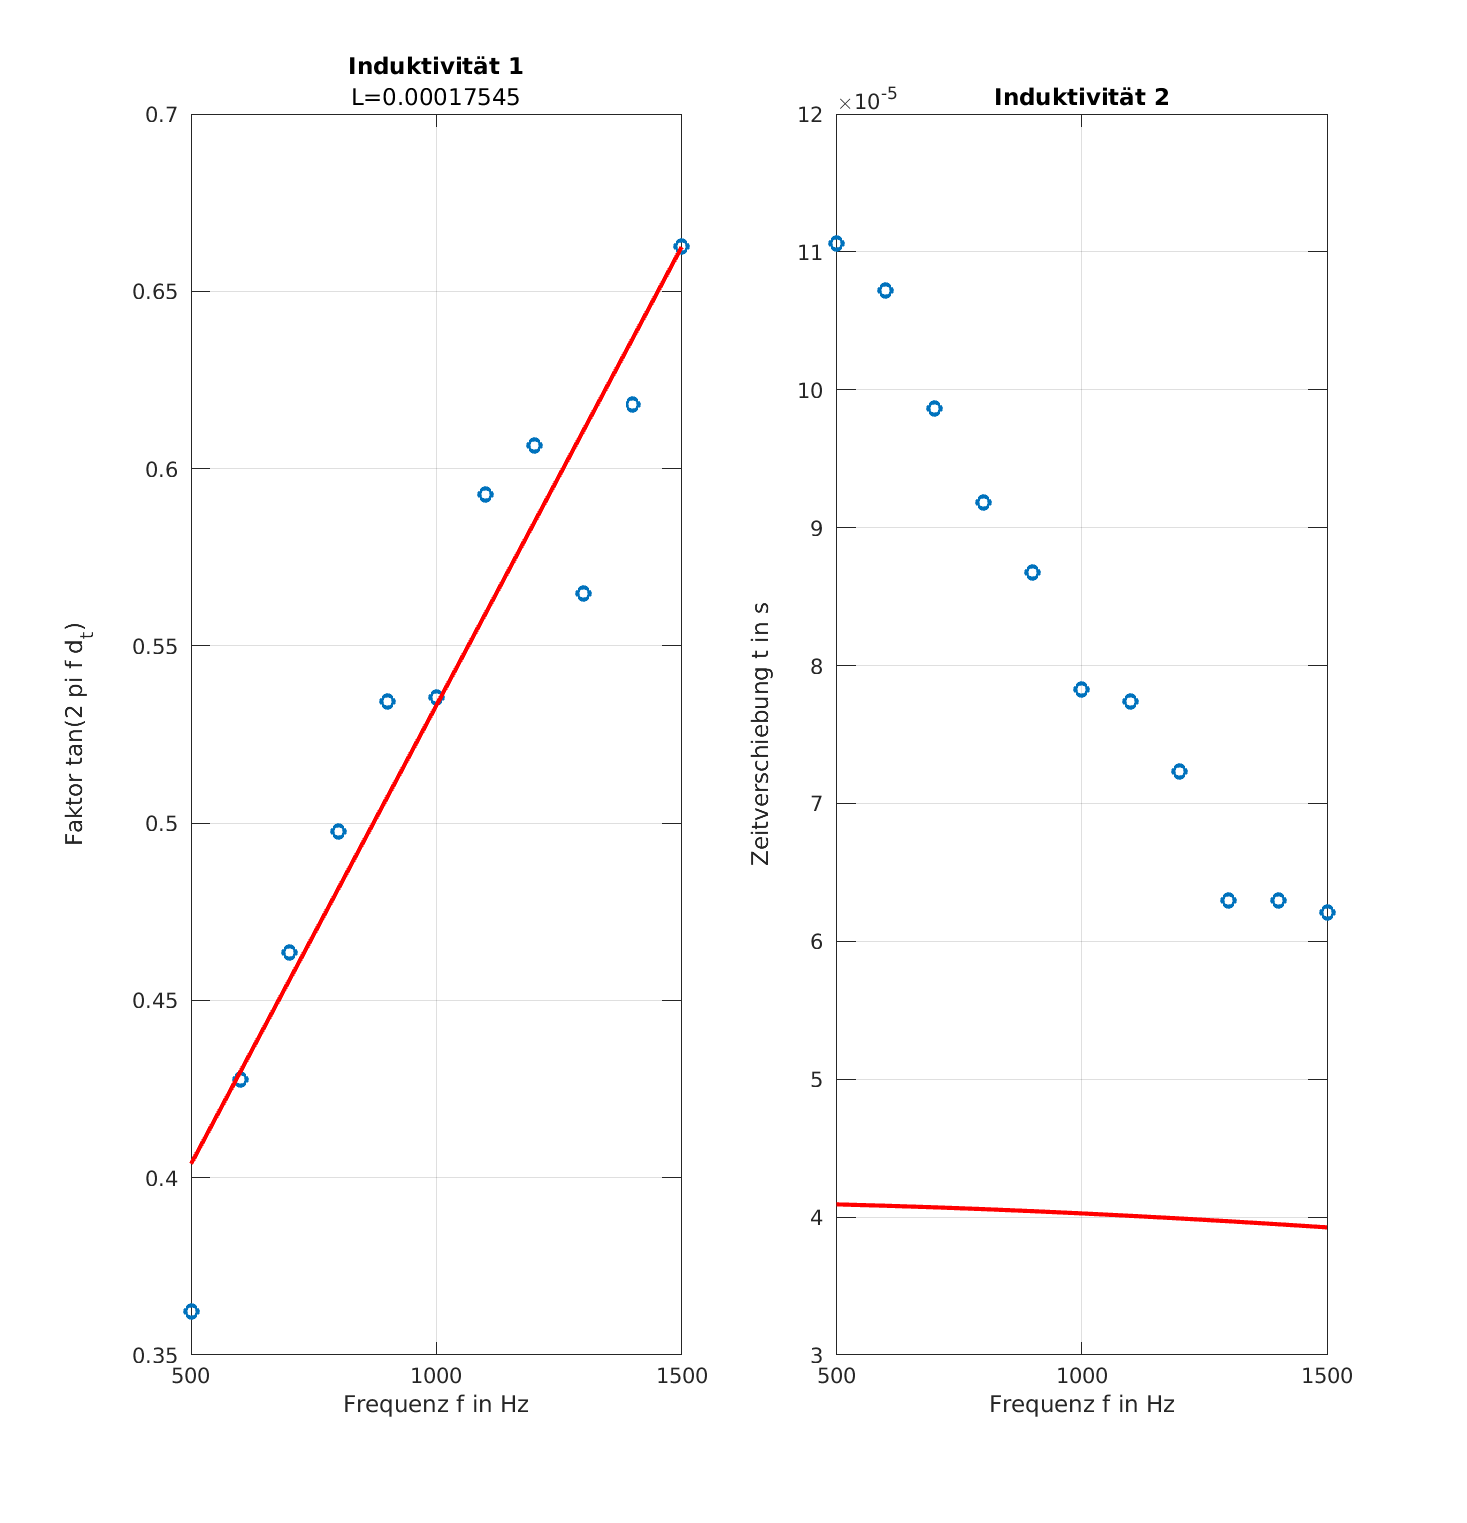
\includegraphics[width=1\textwidth]{as_labor02_1.png}
    \caption{Mess-Schaltung Ankerinduktivität}
    \label{fig:PlotAufgabe1}
   \end{figure}

Diese Schaltung kann durch folgende Maschengleichung beschrieben werden.

\begin{equation} \label{eq211}
    \begin{split}
        u(t)&=u_R(t) + u_L(t)\\
        u(t)&=R \cdot i(t) + L \frac{d i(t)}{dt}\\
        u(t)&= (R+R_s) \cdot i(t) + L \frac{d i(t)}{dt}
    \end{split}
\end{equation}

Die Idee zur Bestimmung der Induktivität ist nun folgende. Die Schaltung
wird mit einer sinusförmigen Wechselspannung betrieben. Über die
Phasenverschiebung der Eingangsspannung und des Stromes kann die Induktivität
bestimmt werden.

\begin{equation} \label{eq212}
    \begin{split}
        \underline{U} = A \cdot e^{\jmath 0}\\
        \underline{I} = B \cdot e^{\jmath \varphi}
    \end{split}
\end{equation}

Der Strom $i(t)$ wird indirekt über den Messwiderstand $R_s= 1\Omega$
bestimmt, da folgendes gilt.

\begin{equation} \label{eq213}
    \begin{split}
        i(t)=\frac{u_{Rs}(t)}{R_s} = u_{Rs}(t)
    \end{split}
\end{equation}

Der Phasenwinkel kann über die Impedanz $\underline{Z}$ berechnet werden.

\begin{equation} \label{eq214}
    \begin{split}
        \underline{Z} &= (R + R_s) + \jmath \omega L\\
        \varphi\{\underline{Z} \} &= \arctan \left( \frac{\omega L}{ R + R_s} \right)
    \end{split}
\end{equation}

Da nicht der Phasenwinkel $\varphi$ sondern die Phasenverschiebung $\Delta t$ gemessen
wird, muss dieser noch umgerechnet werden.

\begin{equation} \label{eq215}
    \begin{split}
        \varphi &= \frac{\Delta t}{T} \cdot 2 \pi \\
        \varphi &=  \omega \Delta t = 2 \pi f \Delta t
    \end{split}
\end{equation}

Nun lässt sich die Induktivität $L$ folgendermaßen berechnen.

\begin{equation} \label{eq216}
    \begin{split}
        L = \frac{(R+R_s) }{2 \pi f} \cdot \tan(2 \pi f \Delta t)
    \end{split}
\end{equation}

Da in der Messung die Phasenverschiebung $\Delta t$ in Abhängigkeit
von der Frequenz $f$ gemessen worden ist, ergibt sich die Funktion $f_1(f)$.

\begin{equation} \label{eq217}
    \begin{split}
       \Delta t = f_1(f) = \frac{1}{2 \pi f} \arctan \left( \frac{2 \pi L}{R + R_s} f \right)
    \end{split}
\end{equation}

Um diese Funktion zu Linearisieren muss diese noch umgestellt werden.

\begin{equation} \label{eq218}
    \begin{split}
       \tan(2 \pi f \Delta t) = f_2(f) = \frac{2 \pi L}{R + R_s} f
    \end{split}
\end{equation}

Nun kann mittels der linearen Regression aus den beiden Vektoren die Steigung
$m$ bestimmt werden, aus der sich die Induktivität $L$ berechnen lässt.

\begin{equation} \label{eq219}
    \begin{split}
       m &=  \frac{2 \pi L}{R + R_s}\\
       L &= \frac{m \cdot (R+R_s)}{2 \pi} \simeq 175.462 \mathrm{\mu H}
    \end{split}
\end{equation}


\begin{figure}[H]
 \centering
    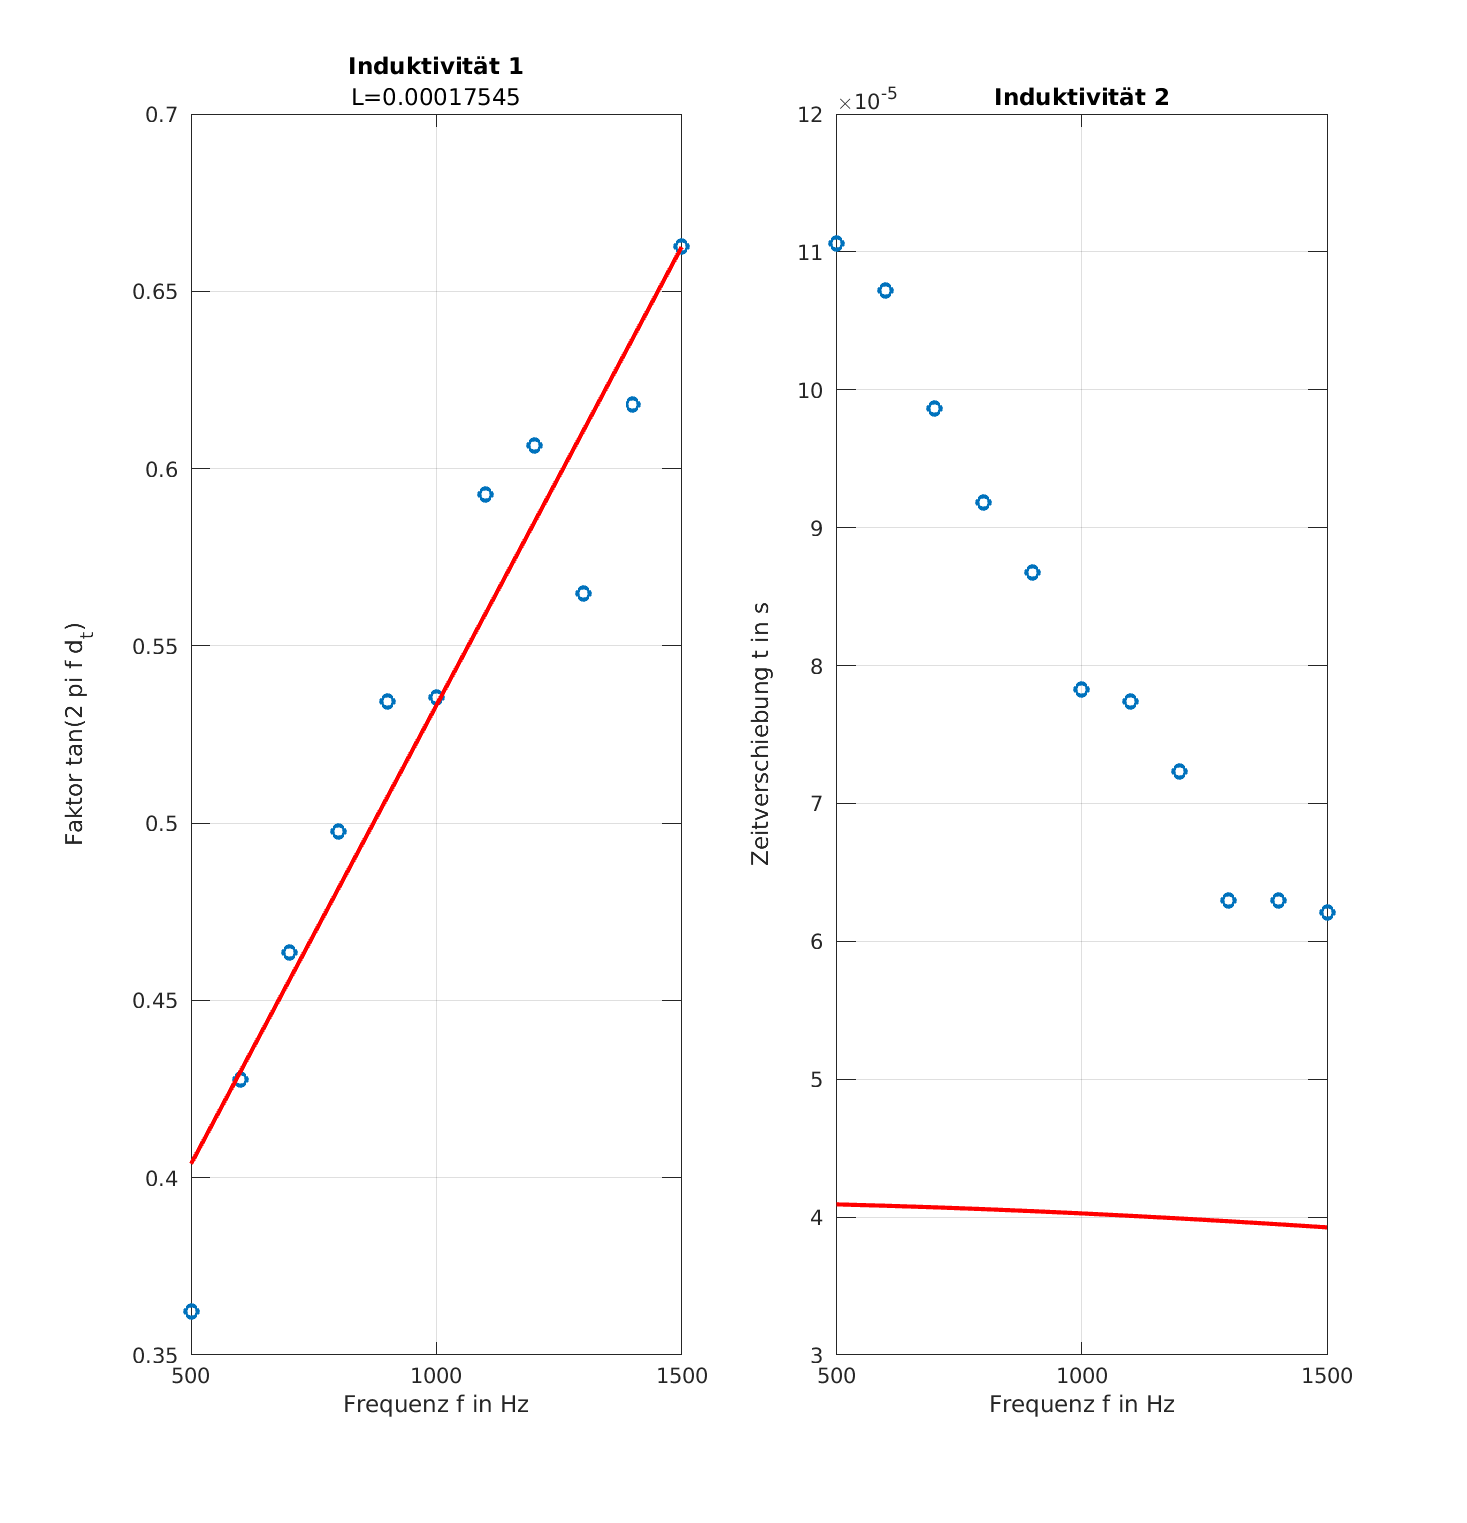
\includegraphics[width=1\textwidth]{as_labor02_1.png}
 \caption{Plot der Aufgabe 1}
 \label{fig:PlotAufgabe1}
\end{figure}